\chapter{実験}
\label{experiment}
%仮説を検証するためにやったことを再現可能な様に書く
%結果も書く

本章では提案手法の実装について述べる。

\section{概要}
\label{sub:実験概要}
本研究の仮説をもとに、システムの実装をおこなった。
\begin{figure}[h]
  \begin{center}
      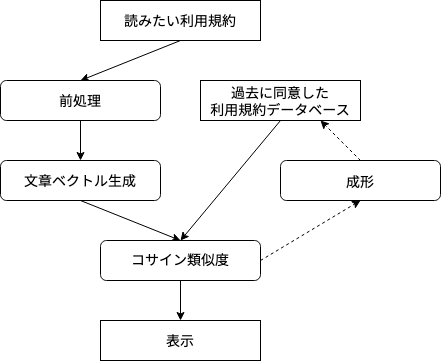
\includegraphics[width=10cm]{img/system.drawio.png}
      \caption{類似条文検出の実装イメージ}
      \label{img:類似条文検出の実装イメージ}
  \end{center}
\end{figure}
図\ref{img:類似条文検出の実装イメージ}に示したように、まず、読みたい利用規約について、前処理を行う。ここでは、URLの置き換え、かっこなどの記号の除去、「利用者」「会員」などを「ユーザー」に表現を揃えるなどの処理を行う。また、条文と条文でない部分(「第○条」、「以上」のような表現など)を除去するための情報がここで与えられる。本研究では、条文でない部分に関しての情報はあらかじめ手作業で与えることとした。その後、文章ベクトルを生成する。本研究では、東北大乾研の大規模日本語モデルを利用した。そして、生成された文章ベクトルと過去に同意した利用規約データベースに保存されている文ベクトルとコサイン類似度の計算を行い、表示する。表示したのち、利用者が同意をした場合は、文章の成形、保存された文章に前処理で取り除けなかった余分な情報などが含まれないかを確認し、必要であれば編集と文章ベクトルの再生成を行い、過去に同意した利用規約データベースに保存する。その情報が増えることにより、検出される条文が増える。同意しなかった場合は保存をしない。

\section{表示方法}
表示方法については、利用規約の類似条文検出に加えて、判断の材料にするために、類似度の高い順に3つの条文とその条文をもつサービス名、コサイン類似度を表示した。3つに設定した根拠としては、他サービスの条文と比較するときに複数サービスの条文と比較することで、より類似度を利用者が比較しやすいと考えたからである。

%\section{実行環境}
%\begin{center}
%  \begin{tabular}{ll} \hline
%    項目 & 仕様 \\ \hline \hline
%    環境 & Azure Web App Service\\
%    インスタンス & B1 \\
%    コア数 & 1 \\
%    RAM & 1.75GB \\ \hline
%  \end{tabular}
% \end{center}

%%% Local Variables:
%%% mode: japanese-latex
%%% TeX-master: "../bthesis"
%%% End:
